% !Mode:: "TeX:UTF-8"
\mychapter{适用于二维码单向传输的硬件以及环境系统}
\label{cha:hd}

本章主要阐述与上一章所实现的基于二维码的图像识别单向网闸的配套硬件及其控制组件与用户界面的介绍。

\section{硬件设计}

硬件设计是本系统的基石。设计要求采用图像识别的方法,涉及到一个编码端和一个解码端。由于是基于摄像头拍摄屏幕这一工作流程进行实际的数据传输,要求物理设备具有很高的稳定性,物理结构必须经过精心设计,且最终成品必须容纳在标准机柜内。

\subsection{显示屏}

编码端的显示屏用于展示编码后的二维码。显示屏的刷新频率不得低于60FPS;响应时间不得高于5ms。显示屏与编码服务器之间采用可靠的有线方式连接,采用HDMI或者DP线缆以提供足够的显示带宽以支持屏幕刷新。

显示器显示面板本身具有自身固有属性:尺寸、分辨率、PPI(像素密度)、亮度、对比度、刷新率、响应时间、面板类型,这些属性均会对传输信道造成实质的影响。由于屏幕本身涉及的参数较多,且难以进行理论分析,亦无法进行控制变量实验。

在项目中,共采购3款显示器:AOCQ27G2S,BENQXL2546K,BOENE156FHM-NZ1,并对他们进行实验分析。使用UFOTest,30Hz Flicker以30Hz为刷新率,将屏幕背景与⽂字在\#000000与\#FFFFFF之间切换。每屏显⽰2位⼗进制,刷 新⼀次数字⾃增1,达到60时不显⽰60⽽回到0。实际数字循环花费60次屏幕刷新,2秒时间。使用Lt-C1950摄像头(162FPS)以1ms曝光时间拍摄刷新过程,得到如下结论:

对于AOCQ27G2S,显⽰器的屏幕刷新时间约为6.4ms,像素灰阶响应时间约为5ms(WtB/GtG最⼤灰阶)。 从显⽰器收到信号,到画⾯被完整呈现在屏幕上,耗时约11ms。 在1ms曝光时间情况下,绝对有效拍摄区间4.7ms。要求摄像头帧率达到213FPS。 超过90Hz刷新率时会使得不存在清晰图像可被拍摄到。 在摄像头为162FPS的情况下,帧间隔6.173ms,保证图像绝对清晰的理论最⼤刷新率为55Hz。

对于BENQXL2546K和BOENE156FHM-NZ1,显⽰器的屏幕刷新时间约为4.1ms,像素灰阶响应时间约为1ms(WtB/GtG最⼤灰阶)。从显⽰器收到信号,到画⾯被完整呈现在屏幕上,耗时约5ms。摄像头为162FPS的情况下,帧间隔6.173ms,保证图像绝对清晰的最⼤刷新率为89Hz。

如上的差异是由显示器面板所决定的(见附录A),基于IPS与VA面板的屏幕像素响应速度不足以支持本项目所要求的高刷新率环境,项目中应当采用大小合适,刷新率满足要求且响应时间低的LCD显示器(主要为TN面板),而不使用CRT、OLED显示器。考虑到机柜尺寸限制,最终选用15.6英寸的BOENE156FHM-NZ1作为显示面板。

\begin{figure}[!htbp]
\centering
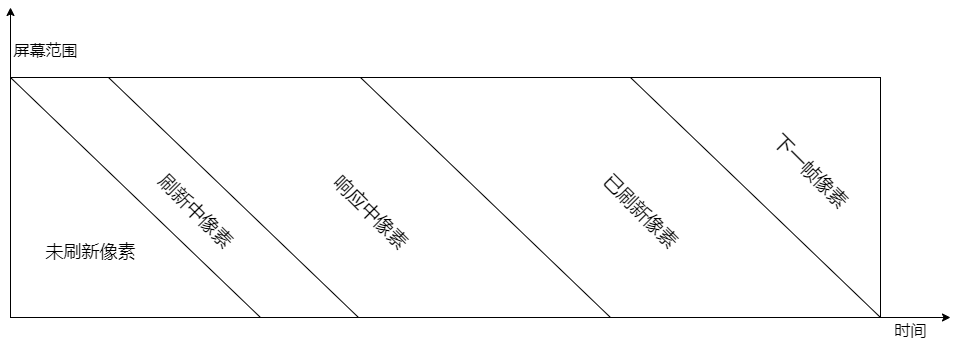
\includegraphics[scale=0.4]{figures/HW/Cap_Pt.png}
\caption{摄像头捕获的显示器刷新过程}
\end{figure}

显示器的面板详细属性参见附录A。

\subsection{摄像头与镜头}

解码端的摄像头用于拍摄展示后的二维码。摄像头的摄像频率不得低于60FPS,最高速率不设上限,但必须不影响功能的实现。摄像头应采用标准的网口或者USB接线传输数据,数据传输的带宽应当能够支持最高速拍摄时的数据速率。内部如有采用独立开发的接口的,必须提供合适的转接层,保证普通的计算机能直接通过网口或USB接线连接上摄像头。

需要调节摄像头的一系列参数从而得到屏幕图像的清晰图案。具体参数包括:光圈、感光度、曝光时间、增益、白平衡。摄像头所能拍摄的分辨率决定了拍摄图像对原始屏幕输出的解析能力,帧率决定了对屏幕图像的获取速度。二者直接制约接收端的接收带宽。

假定屏幕刷新率120FPS,则每1/120=0.0083=8.3ms,屏幕刷新一次。考虑到屏幕有响应时间(前一帧淡出,后一帧淡入),考虑2ms的情况(实际会有所偏差),屏幕的图像特性如图5.2所示。

\begin{figure}[!htbp]
\centering
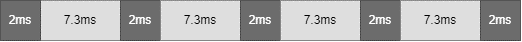
\includegraphics[scale=1]{figures/HW/Rf_Model.png}
\caption{显示器刷新模型}
\end{figure}

显然我们不希望在红色区的响应时间内拍照,因此就需要Lock-in同步。然而,也可以通过如下的两个逻辑解同步:

1.如果落在响应时间内,算法要能认识到这一点并抛弃一帧

2.下一帧一定落在本帧的非响应时间内

第一点,可以用纯色定位块解决。因为8张二维码不会堆满整个屏幕,所以我们可以在某一个区域放置纯色的定位块。接下来,我们为连续的三帧分别给上红绿蓝三种纯色定位块,称之为红帧、绿帧和蓝帧。考虑相机现在拍摄完红帧,这样,算法知道下一帧是绿帧。如果屏幕现在处于响应时间,定位纯色块要么是暗淡的灰色,要么是红绿之间的黄色,总之不会是纯绿色。因此,按照某种绿色阈值,可以检测并抛弃一帧。

第二点,如果我们使用150FPS的相机,则每1/150=0.0066=6.6ms,拍摄一张照片。考虑拍照时间落在响应时间内的两种极限情况(黄色和绿色标出),下一帧都一定会落在本帧的非响应时间内,从而得到正确的成像。摄像头采集的模型如图5.3所示。

\begin{figure}[!htbp]
\centering
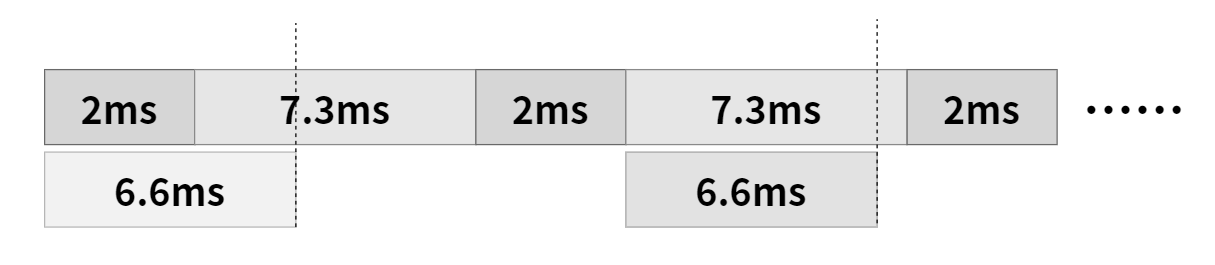
\includegraphics[scale=0.4]{figures/HW/Cap_Md.png}
\caption{摄像头采集模型}
\end{figure}

项目中摄像头采用Teledyne Lumenera Lt-C1950 Pregius Global Shutter CMOS USB3 Camera作为首选摄像头,其提供了1936 X 1216分辨率(230万像素)下162FPS高速实时图像传出。外形尺寸为45毫米x 45毫米x 36.1毫米,较为小巧,满足设计需求。

\begin{figure}[!htbp]
\centering
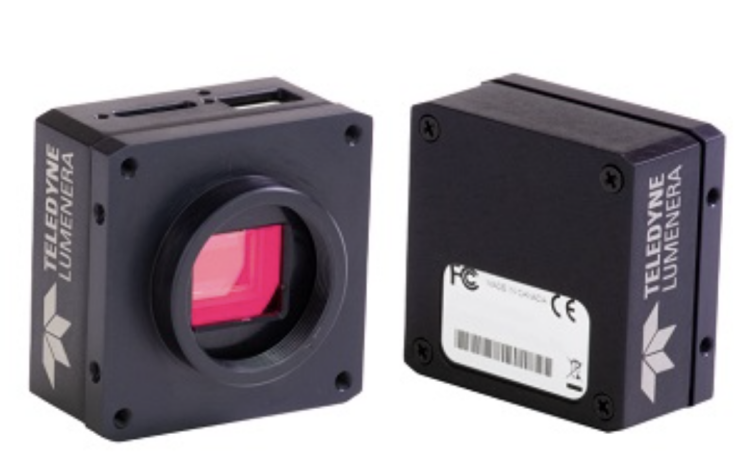
\includegraphics[scale=0.6]{figures/HW/LTC1950.png}
\caption{Lt-C1950摄像头}
\end{figure}

镜头的基本功能是光线转换(调制)。在视觉系统中,镜头的主要功能是将目标成像于相机的CMOS或是CCD上。镜头的好坏直接影响到系统的整体性能,合理选择与安装镜头是视觉系统设计与实施的一个重要组成部分。\cite{郑新宇0基于视觉检测的对位贴合系统设计与应用}

定焦镜头的主要调节参数为焦距与光圈。焦距越小,景深越大,畸变越大,渐晕现象越严重,使像差边缘的照度降低; 光圈越大,图像亮度越高,景深越小。\cite{刘混海2009基于机器视觉的集成芯片基板定位技术研究}

使用焦距小的镜头可以帮助减小整套光学传输模块的尺寸,但代价是获得的图像将有更明显的鱼眼效应与暗角。

项目中采用的镜头为500万像素1/1.8英寸VM0420MP5 4mm C口镜头。

\begin{figure}[!htbp]
\centering
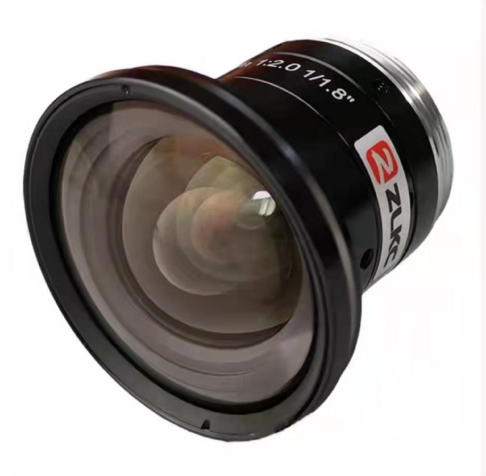
\includegraphics[scale=1.4]{figures/HW/VM0420MP5.png}
\caption{VM0420MP5镜头}
\end{figure}

受制于摄像头与屏幕之间的距离因素,一个摄像头无法捕捉到整个屏幕的完整画面。在本项目中使用两个独立摄像头拍摄同一块屏幕的不同区域。

\subsection{机架}

摄像头与屏幕固定在主承载支架上,保证摄像头与屏幕在工况下相对位置不发生变化。摄像头可以通过可靠的夹具夹持,显示器可以使用符合VESA标准的支架进行固定。主承载支架应当具有减震与避震措施,避免微振动对图像识别造成的影响。摄像头与解码服务器的数据线连接需要使用可靠的锁止装置,如果使用USB外形的接口,应当附加数据线与摄像头本体的锁扣链接;如果使用RJ-45外形的接口,需要确保水晶头的锁定可靠性。显示器与编码服务器的连接同样需要保证可靠性。VGA与DVI不足以承受系统所需要的显示带宽,故不使用。应当使用附加锁扣装置的HDMI数据线或者全尺寸DP接口的数据线(全尺寸DP接口自带锁止装置)。镜头可以通过C口连接到摄像头。如果采用定焦摄像头,则镜头的对焦转盘与光圈转盘应当安装有限位器,保持焦距与光圈的固定。

为避免环境光对系统运行产生的干扰,整个光学传输模块需要有完整的不透光蒙壳。蒙壳内侧(即光学传输模块运行的一侧)需要使用深色哑光材质,使得蒙壳自身的干扰降到最低。蒙壳内需要有一定的热量交换途径,防止摄像头与显示屏超出工作温度。如果采用风冷的方式,需要安装额外的空气滤清装置避免外部异物入侵到蒙壳内。机箱整体的尺寸(单位:mm)约为470(w)*800(l)*350(h),机箱内部的设计以及真实硬件如图5.6与图5.7所示。

\begin{figure}[!htbp]
\centering
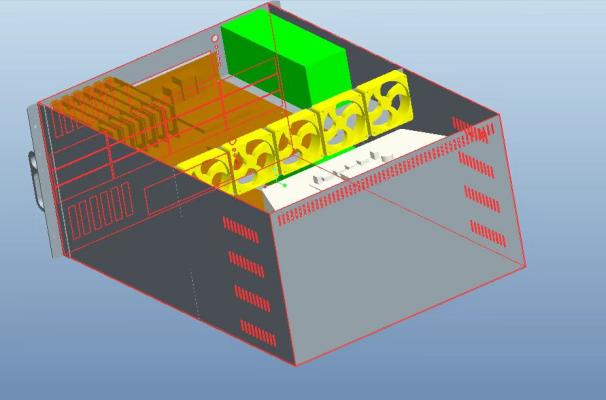
\includegraphics[scale=1.6]{figures/HW/Design.png}
\caption{服务器设计}
\end{figure}

\begin{figure}[!htbp]
\centering
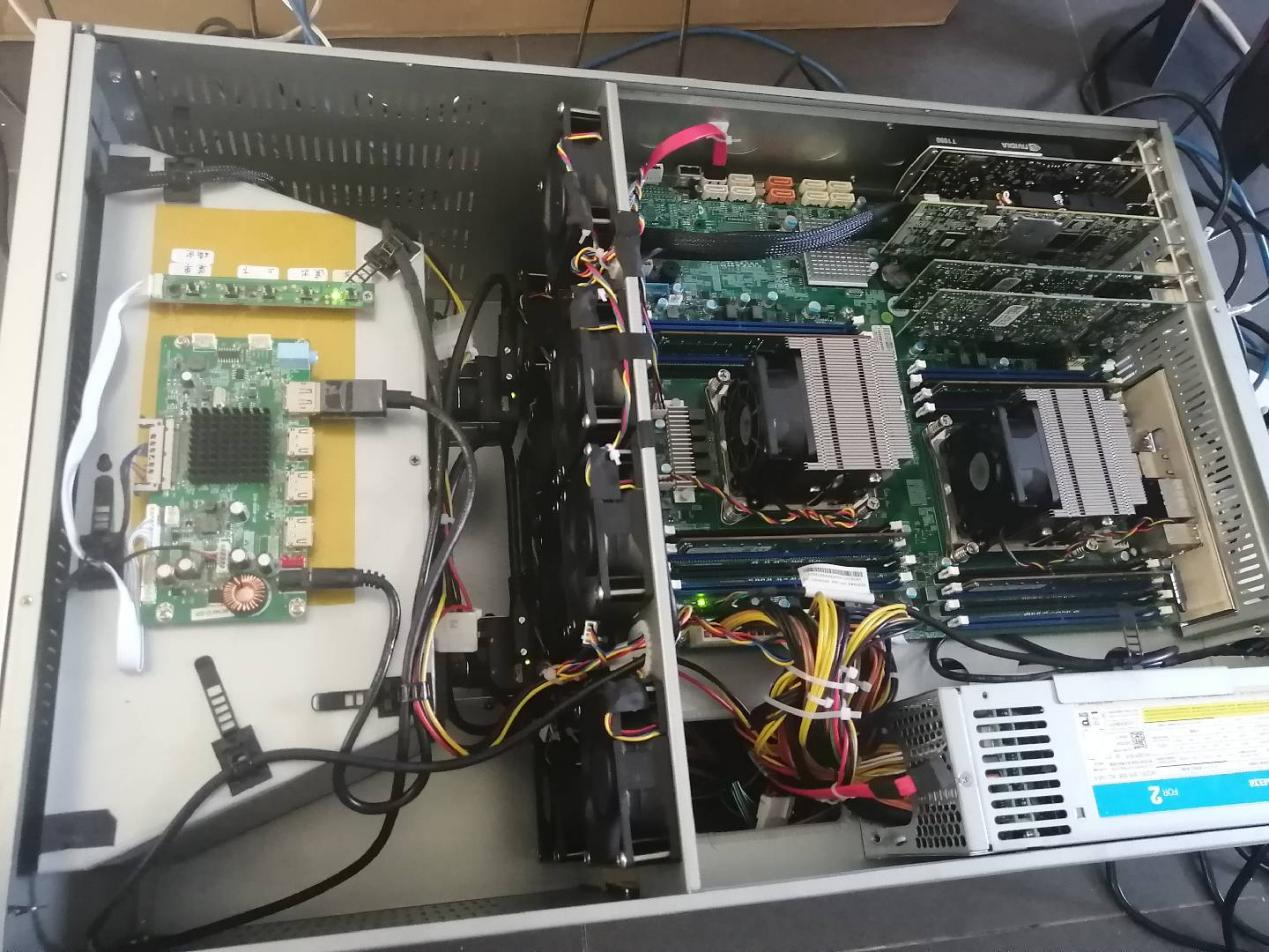
\includegraphics[scale=1]{figures/HW/Real_HW.png}
\caption{服务器硬件}
\end{figure}

服务器的硬件参数如表5.1,表5.2所示

\begin{table}[htb]
  \centering
  \begin{minipage}[t]{0.8\linewidth} 
  \caption[硬件参数]{硬件参数}
    \begin{tabularx}{\linewidth}{lX}
      \toprule[1.5pt]
      {\heiti 技术参数} & {\heiti 指标} \\\midrule[1pt]
      CPU    & INTEL E5 2699V4 *4 \\
      GPU    & NVIDIA T1000*1  NVIDIA T300*1 \\
      RAM    & 2*4*32GB \\
      存储   & 2*2*1000GB SSD RAID1系统盘,2*4*6TB HDD RAID5数据盘 \\
      网络接口    & 8*RJ45 千兆以太网网口 \\
      管理接口    & 2*RJ45 千兆以太网接口 \\
      USB    & 4*USB2.0 4*USB3.2Gen1 \\
      \bottomrule[1.5pt]
    \end{tabularx}
  \end{minipage}
\end{table}

\begin{table}[htb]
  \centering
  \begin{minipage}[t]{0.8\linewidth} 
  \caption[物理与电气特性]{物理与电气特性}
    \begin{tabularx}{\linewidth}{lX}
      \toprule[1.5pt]
      {\heiti 技术参数} & {\heiti 指标} \\\midrule[1pt]
      输入电源    & 100-240V 50-60Hz AC \\
      多电源输入    & 双电源冗余 \\
      功率    & 550W*2 \\
      过载与冗余保护  & 支持 \\
      尺寸(WxDxH) & 444*750*250mm \\
      重量(kg) & 50 kg \\
      散热设计 & 风冷 \\
      安装方式 & 19英寸6U机架 \\
      工作环境 & -10℃ ~ +40℃ ,5\% ~ 90\%无凝结 \\
      存储温度 & -20℃ ~ +60℃ ,5\% ~ 95\%非凝结 \\
      IP防护等级 & IP30 \\
      \bottomrule[1.5pt]
    \end{tabularx}
  \end{minipage}
\end{table}

\section{周边控制组件}

在有数据传输的能力之后,我们还需要对整个系统进行一定程度的控制,以更好地满足业务上的需求。

\subsection{网络与时间模块}

网络模块提供了配置系统网口,驱动Socket程序的能力。

网络模块提供了可以直接操纵系统级别网口配置的能力,在用户需要重新配置网络环境时,通过web应用或修改数据库的方式将配置文件存入MySQL的配置表中,发出网络配置指令后,网络模块会生成新的yaml配置文件,使用NetPlan的接口将新的配置作用于NetworkManager,然后对系统的配置作出修改。网络模块同时支持对ICMP报文的处理规则应用。

网络模块旨在提供易用的、即时生效的、重启不改变的网络环境配置,为配置静态IP、禁止ping服务等需求提供服务。网络模块生效的实现流程如图5.8所示。

\begin{figure}[!htbp]
\centering
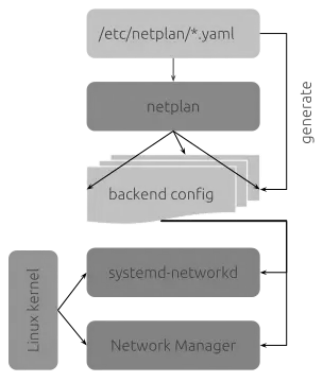
\includegraphics[scale=1]{figures/HW/N1.png}
\caption{网络配置流程}
\end{figure}

本系统提供NTP在不连接外网的情况下提供可靠的时间服务。

网络时间协议NTP用来使客户端和服务器之间进行时钟同步,提供高精准度的时间校正。NTP依赖从客户端到服务器的往返延迟delay,客户端与服务端之间的时间差offset来计算调整自己的时钟,实现与NTP服务器的时钟同步。

\subsection{IP白名单模块}

IP白名单模块提供了传输机别的基础安全机制,使用白名单方式保证传输的安全性。

对于编码侧与解码侧,IP白名单分别作用于两侧的Socket程序,只接受白名单IP发送的数据,只将数据发送给白名单内的IP。IP白名单存储允许连接的IP地址,在建立连接时检查来源地址/目标地址是否在白名单中,而后允许或者拒绝连接。

编码端的IP白名单检查发生在socket连接建立的过程中。对于发送到编码器的TCP或UDP请求,可以获知来源的IP地址,如果IP地址不在白名单中则直接断开当前连接。解码端的IP白名单发生在socket连接建立之前。由于总是由解码器进行连接的发起,对于不在IP白名单内的目的地址,不会尝试进行连接的建立。处理流程如图5.9所示。

\begin{figure}[!htbp]
\centering
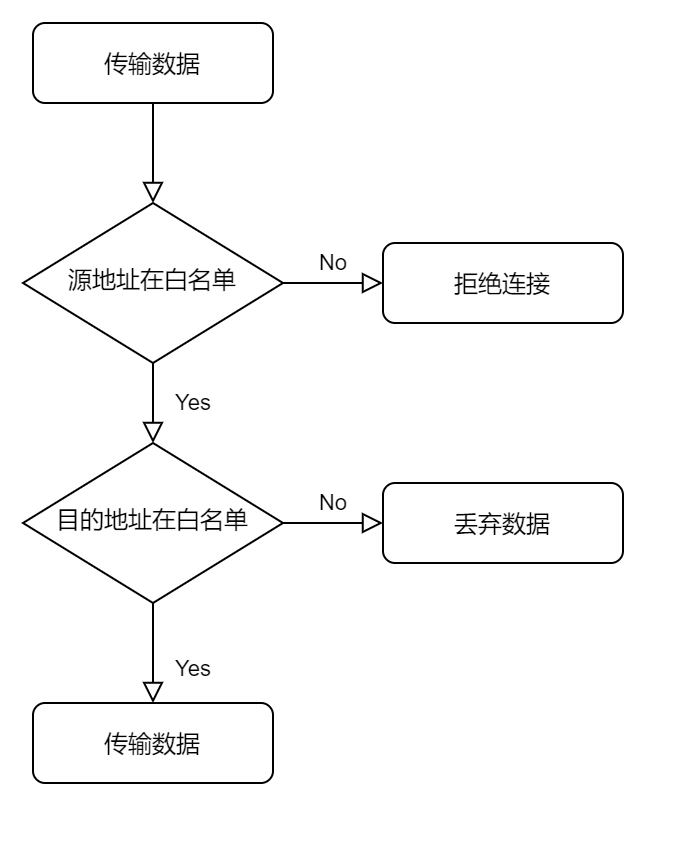
\includegraphics[scale=0.4]{figures/HW/N2.png}
\caption{IP白名单}
\end{figure}

IP白名单模块提供IP白名单的增删改查功能。通过该模块,用户可以便捷的对IP白名单进行各种必需操作,并实时的反映在整个传输系统上。IP白名单为单向隔离系统提供传输级别的IP地址过滤,是系统安全性的重要组成部分。

\subsection{用户模块}

本产品支持三权分立,内置配置员、审计员、管理员三个用户。

配置员:用于网络与用户配置。

审计员:用于事件日志审计。

系统管理员:用于系统管理。

通过用户模块,可以完成用户名单的增删改查工作,可以根据用户名与密码正确的进行用户的验证,可以在连续多次密码错误时对账号进行冻结,可以做到冻结时长与密码错误次数的联动,可以在超出冻结时长后自动对用户进行解冻,可以手动的对用户进行解冻,对不同权限的用户可以正确的接收、拒绝对应的操作。

本项目基于RBAC(基于角色的权限控制)模型进行权限管理。在本系统中,共预制有配置、审计、管理三种角色。不同的角色对应了不同的权限。

系统支持子菜单级别的用户管理。通过用户管理功能,可以创建若干角色并分配权限,创建用户时可以直接授权该角色的权限。对于已经创建的用户,可以进行修改与删除操作,支持修改的内容包括帐号、密码、权限等。

项目采用帐户密码认证+jwt方式验证用户的登录状态,token的失效期为1小时。所有前端请求会经过拦截器,再由后端验证token。用户在登录界面成功登录后 获取token,验证权限,而后用相应权限访问对应接口获得数据或者执行操作。Token采用SHA256算法加密。在无token、token过期、用户验证错误等情况下,会拒绝用户所做查询与操作。通过用户认证机制,可以依据权限做用户操作加以限制。

为了防止恶意使用者通过暴力枚举的方式破解用户密码,在短时间连续多次密码错误后会对用户进行冻结。在用户连续3次密码错误后,每一次失败的登录尝试会将账户的冻结时间累加3分钟。在冻结时间超时后,账户会自动解冻。管理员亦可以手动对指定的账户进行解冻操作。

\subsection{日志、数据缓存与流量统计}

本系统提供多种日志记录,提供完整的数据缓存以及持久化,提供基于缓存数据的流量统计。可以依照时间、分类、级别、关键词准确的查询对应的日志项,各个系统的关键操作可以被正确的记录到日志库中。

系统日志记录系统级别操作日志,包括NTP操作,端口初始化等。通过查询或审计系统日志,可以对系统运行状态以及历史操作进行审计。

警告日志记录系统运行时出现的各种错误情况,包括系统内部的传输错误、目的地址不可达、文件模式不符合等。

登录日志记录用户的登录操作,包括登录成功与登录失败的记录,便于管理员判断用户行为模式,及时对异常情况做出操作。

操作日志记录对于系统所做的一系列配置操作,包括网络配置、用户配置、IP白名单配置等。用户所做出的重要操作均会被记录于操作日志中。

由于系统存在严格的单向性,对于解码器出现的错误,编码器完全无法获知,使得整个系统无法提供严格意义的可靠传输,只能提供尽最大可能的无差错传输。如果出现问题,需要借助外力介入进行恢复或重传,对于时间段内的数据,将它们进行暂存是一种较好的方式。但是对于成功的传输,系统亦无法得知其具体的传输情况。因而采取对所有的传输全部暂存的方式。

对于所有的传输,基于Linux系统“一切皆文件”与单向网闸的设计,接受到的数据流会首先以文件形式进行缓存、传输,对于传输完成的文件,会根据传输信息与传输状态,将文件移动到对应的备份路径下进行保留。如果后期需要恢复文件,可以根据传输的网口号、协议、传输时间进行对应的查找。

所有发送数据的内容部分,会以原始二进制形式进行数据备份。存储时不指定特定格式,统一作为比特流处理,存储为无后缀元文件。存储以入库网口-协议-精确到纳秒的传输发生时间作为文件名,便于数据的查找与恢复。记录保存6个月。

在流量统计模块中,可以查看流量总览和设备流量趋势。

流量统计主要包含主要包含了流量总览和端口流量两个部分。流量总览显示设备总的流量数据和根据协议分类汇总的数据。端口流量按端口号显示流量数据。

流量总览可以依据协议,以分钟或小时作为时间单位显示过去10个时间段的传输流量以及传输条数。端口总览可以依据端口号,以分钟或小时作为时间单位显示过去10个时间段的传输流量以及传输条数。

传输流量可以记录每一个传输的发包数以及传输条数,传输流量可以根据时间段、协议、网口号、IP、端口等,显示符合内容的每一条传输的传输数据量以及发包数,一并包括精确到毫秒的传输时间、传输的IP地址与端口号、协议等一系列审计相关内容。

\section{用户界面}

在本系统中,还提供易于操作的Web管理界面,对整个传输系统进行配置。

项目服务端由Django4构建,使用MySQL作为数据库,并用Redis做一层缓存。项目前端由VUE实现。具体的前后端接口列表见附录B。

\subsection{登录与用户管理}

用户访问编码器的前端地址会被自动路由至登录页面,在编码器的登录页面有用户的登录操作的接口,分别为编码器用户的用户名和密码。其中编码器用户的账号分为管理员权限,审计权限和配置权限。在登录界面没有用户的注册功能,用户的账号的密码为拥有管理权限的管理员账号使用添加用户功能完成。

登录界面分为登录错误和登录成功两种提示,当登录成功时,用户会被自动跳转至该编码器登录用户所对应权限可访问的功能页面。每个用户在密码输入和用户名不匹配时会提示登录错误,每个用户的登录错误次数超过三次时,该账户会被锁定,用户需要联系在系统中管理员权限的账号持有者,通过管理员权限中的解冻锁定账户的功能重新获得该账户的使用权限。登录界面如图5.10所示。

\begin{figure}[!htbp]
\centering
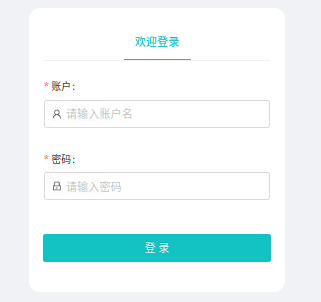
\includegraphics[scale=1]{figures/HW/N3.png}
\caption{用户登录}
\end{figure}

用户配置可以由拥有管理员权限的用户更改解码器中用户的信息。该页面包括以下功能:用户添加,修改用户信息和删除用户。在该页面展示系统中所有用户的信息。包括用户的序号。用户姓名、该用户的权限、该账号的状态、该用户的密码、该用户的账号上述信息。配置界面如图5.11所示。

\begin{figure}[!htbp]
\centering
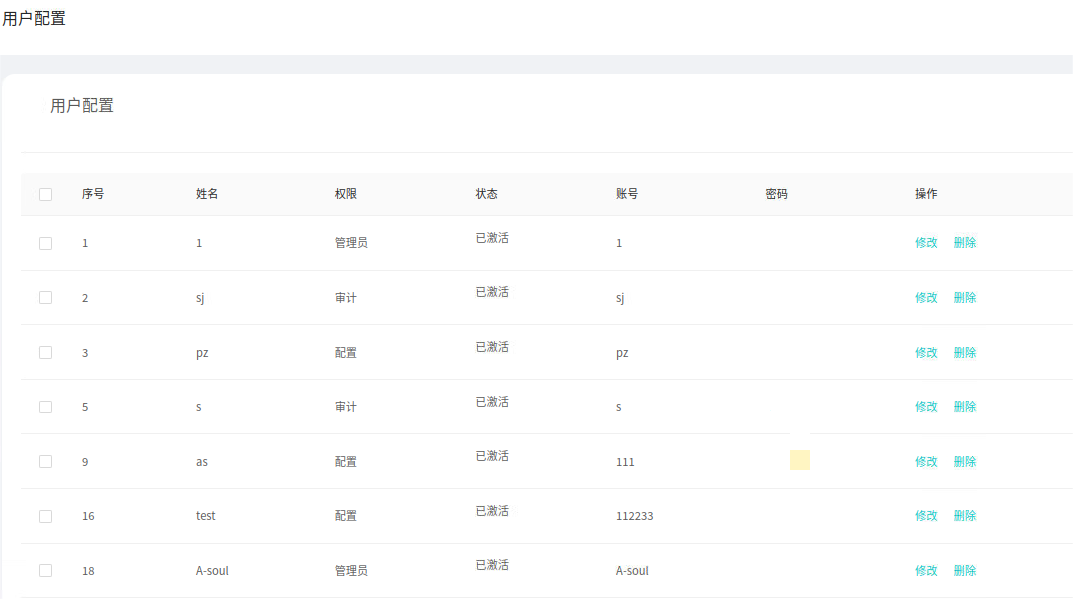
\includegraphics[scale=0.5]{figures/HW/N4.png}
\caption{用户管理}
\end{figure}

\subsection{展示页}

传输展示由展示传输统计和展示产品信息以及展示设备状态等三部分功能完成,系统状态均为实时更新。通过展示页面可以使用户更好的对系统的运行状况进行了解。

编码器传输统计分成两部分主要功能,别分为分开统计编码器的实时传输数据量,和实时传输数据的条数,而统计的功能又分为每小时的数据统计和每分钟的数据统计。同时系统可以选择不同的网口展示来自每个网口的单独统计数据,该网口由实际的接入编码器的网口控制,网口信息可以在网络管理章节中查看,并定义。

本页面所展示的所有数据都分为监听前七个时刻的数据,分别由小时和分钟两种请求方式,在本页面中两个矩形框的右上角分别设有两个下拉选项,该选项框可操控显示矩形框中所请求的实时传输数据为分钟时刻/小时时刻,矩形框内会根据所请求的数据进行图形绘制和数据可视化。

编码器的展示数据功能分别为TCP协议和UDP协议分开展示,图5.12中该页面的蓝色矩形展示框为TCP数据展示界面,绿色矩形展示框为UDP数据展示界面。

\begin{figure}[!htbp]
\centering
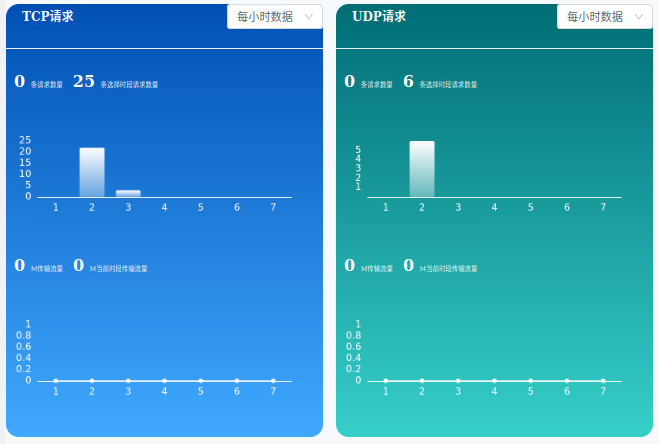
\includegraphics[scale=1]{figures/HW/N5.png}
\caption{数据展示}
\end{figure}

蓝色矩形的上方半部为请求TCP数据的条数的统计展示,分别展示前七个时刻的统计TCP数据,并绘制折线图和柱状图。在所展示的图形的上方为当前一个时刻的TCP数据和前七个时刻TCP数据的总和。蓝色矩形的下方半部为请求TCP数据的流量大小的统计展示,分别展示前七个时刻的统计数据,并绘制折线图和柱状图。在所展示的图形的上方为当前一个时刻的数据和前七个时刻数据的总和。

绿色矩形的上方半部为请求UDP数据的条数的统计展示,分别展示前七个时刻的统计UDP数据,并绘制折线图和柱状图。在所展示的图形的上方为当前一个时刻的UDP数据和前七个时刻UDP数据的总和。绿色矩形的下方半部为请求UDP数据的流量大小的统计展示,分别展示前七个时刻的统计数据,并绘制折线图和柱状图。在所展示的图形的上方为当前一个时刻的数据和前七个时刻数据的总和。

设备状态展示分为展示解码器CPU的状态,内存状态和硬盘状态。该三个硬件设备的状态为每秒钟实时更新的设备状态,如图5.13所示。

\begin{figure}[!htbp]
\centering
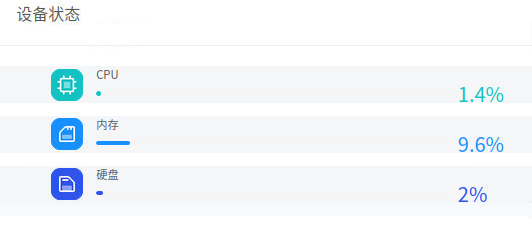
\includegraphics[scale=1]{figures/HW/N6.png}
\caption{设备状态}
\end{figure}

\subsection{网络管理}

网络配置模块提供易用的网络配置抽象,使得用户可以较为便捷的做出系统级别的网络配置更改。

在编码器管理口配置中,管理口的参数分为,IP,网口,子网掩码,网关,web服务,ping服务等属性。编码器的所有管理口的配置将会展示在该页面。在该页面的管理口展示中,拥有网络管理配置权限的用户可以通过展示界面的编辑按钮来修改管理口的配置。管理口的配置界面如图5.14所示。

\begin{figure}[!htbp]
\centering
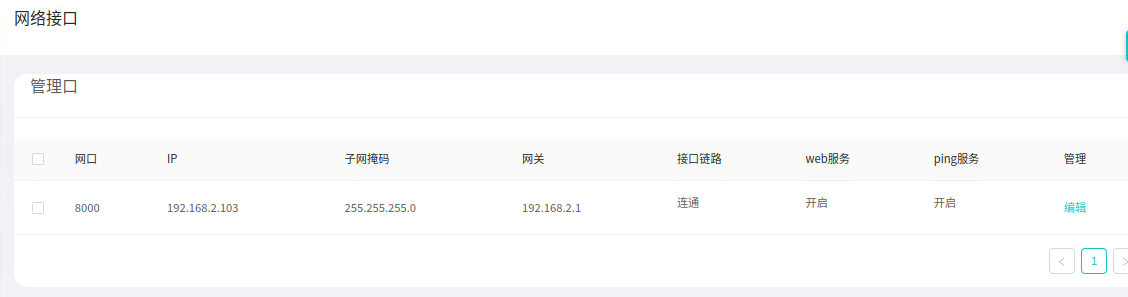
\includegraphics[scale=0.6]{figures/HW/N7.png}
\caption{管理口管理}
\end{figure}

在编码器业务口配置中,业务口的参数分为,网口,入口端口,子网掩码,网关,协等上属性。编码器的所有业务口的配置将会展示在该页面。在该页面的业务口展示中,拥有网络管理配置权限的用户可以通过展示界面的编辑按钮来修改业务口的配置。业务口配置界面如图5.15所示。

\begin{figure}[!htbp]
\centering
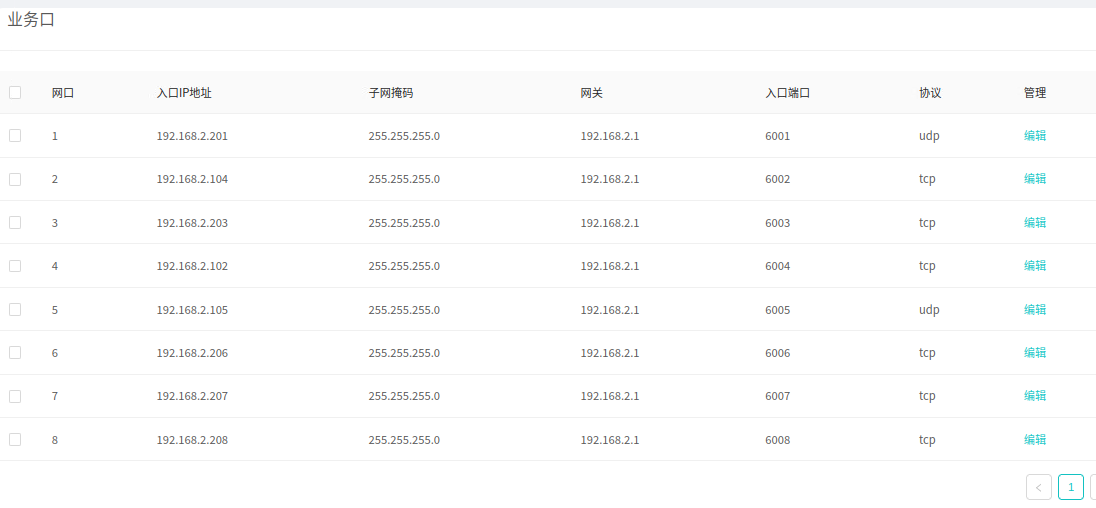
\includegraphics[scale=0.6]{figures/HW/N8.png}
\caption{业务口管理}
\end{figure}

在解码器管理口配置中,管理口的参数分为,IP,网口,子网掩码,网关,web服务,ping服务等属性。解码器的所有管理口的配置将会展示在该页面。在该页面的管理口展示中,拥有网络管理配置权限的用户可以通过展示界面的编辑按钮来修改管理口的配置。管理口的配置界面如图5.16所示。

\begin{figure}[!htbp]
\centering
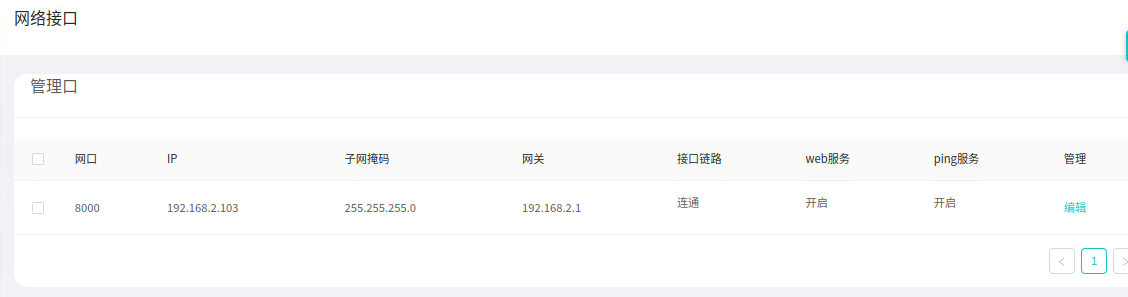
\includegraphics[scale=0.6]{figures/HW/N9.png}
\caption{管理口管理}
\end{figure}

在解码器网口配置中,网口的参数分为,IP,网口,子网掩码,网关,以上属性。解码器的所有网口的配置将会展示在该页面,网口的展示效果如图5.17所示。

\begin{figure}[!htbp]
\centering
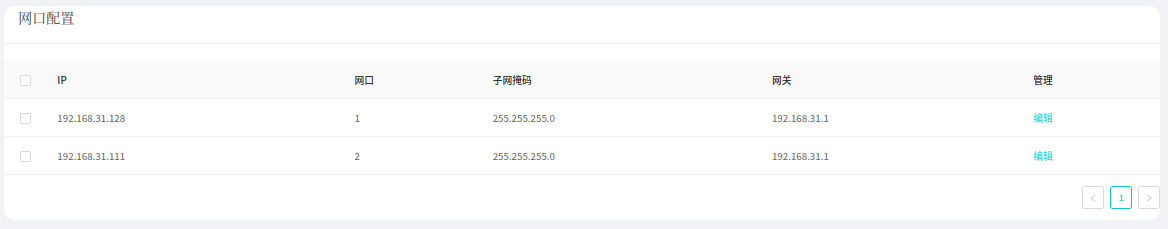
\includegraphics[scale=0.6]{figures/HW/N10.png}
\caption{网口管理}
\end{figure}

在解码器业务口配置中,业务口的参数分为,网口,出口网口,目的IP,目的端口,目的IP协议,子网掩码,网关等属性。解码器的所有业务口的配置将会展示在该页面,在该页面的业务口展示中,拥有网络管理配置权限的用户可以通过展示界面的编辑按钮来修改业务口的配置。业务口的展示效果如图5.18所示。

\begin{figure}[!htbp]
\centering
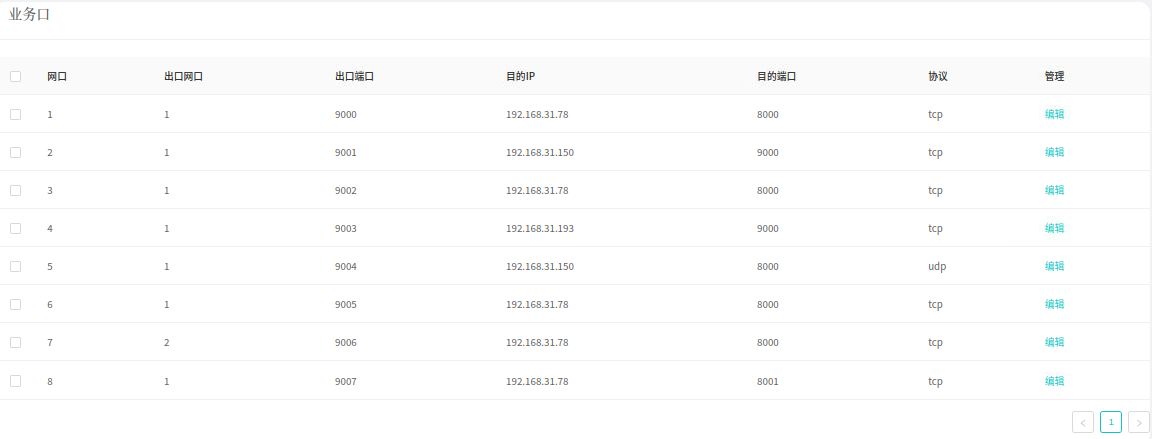
\includegraphics[scale=0.6]{figures/HW/N11.png}
\caption{业务口管理}
\end{figure}

业务口的配置目的是形成一张路由表,完成单向网闸的端口映射以及转发。各个配置的关系如图5.19所示。

\begin{figure}[!htbp]
\centering
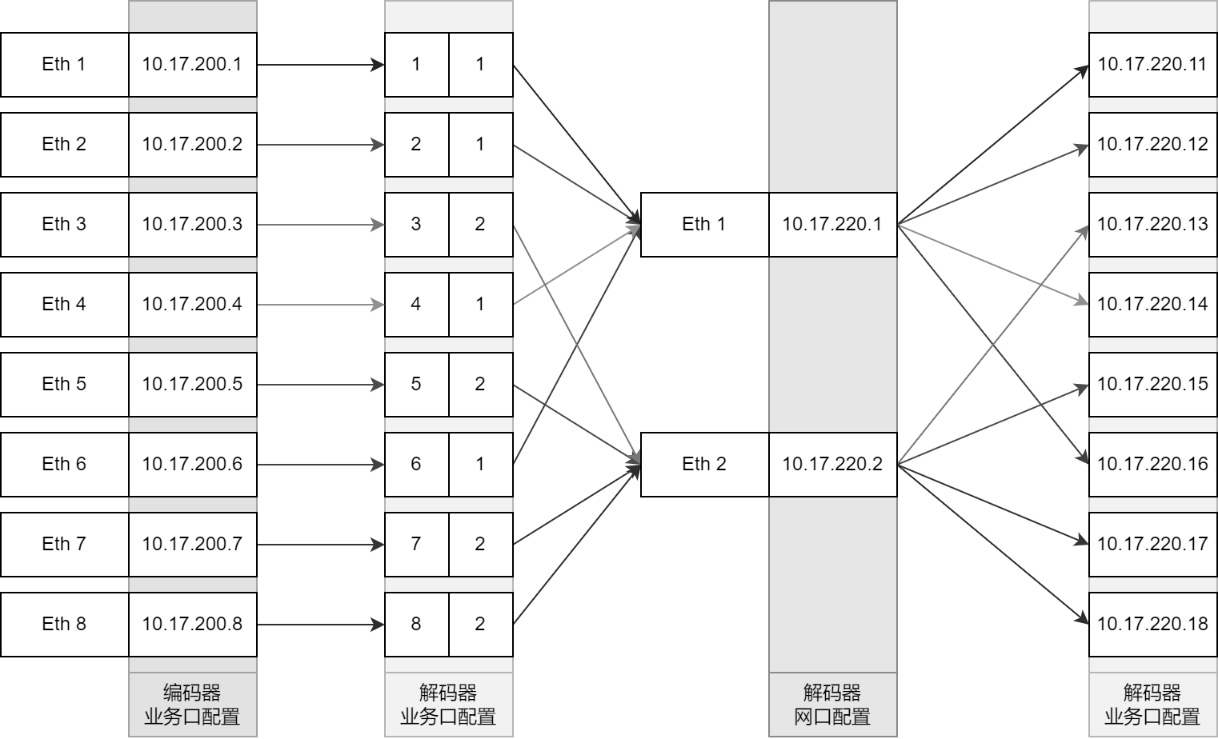
\includegraphics[scale=0.4]{figures/HW/N12.png}
\caption{各个配置之间的关系}
\end{figure}

\subsection{数据缓存与日志}

通过数据缓存和日志模块,我们可以对系统传输的内容以及发生的时间进行追溯,保证系统的安全性,及时发现系统漏洞。

数据缓存界面可以查看详细的历史传输数据。数据缓存页面分为查询部分和数据展示部分。查询部分为图中的上半部分,用户可通过输入源IP、目的IP、使用传输协议、开始时间和结束时间五个参数来查询解码器系统中的历史传输数据。其中源IP、目的IP需要用户手动输入,所使用传输协议是一个下拉框,用户可选择查看TCP协议和UDP协议,开始时间和结束时间是通过日历选择实现,用户可以通过一个下拉日历选择需要查询的数据时间跨度。用户也可以通过日历中的此刻按钮来选择操作时间为需要的时间。查询成功后系统会提示查询成功。

数据查询接口为模糊查询,这意味着用户不需要输入全部的属性作为查询的参数,可以通过输入部分属性进行查询。例如,用户仅输入源IP和目的IP这两个查询参数,这意味着得到的结果是满足这两个查询参数的所有数据。此处的重制按钮可以清除用户已输入的查询参数。查询界面如图5.20所示。

\begin{figure}[!htbp]
\centering
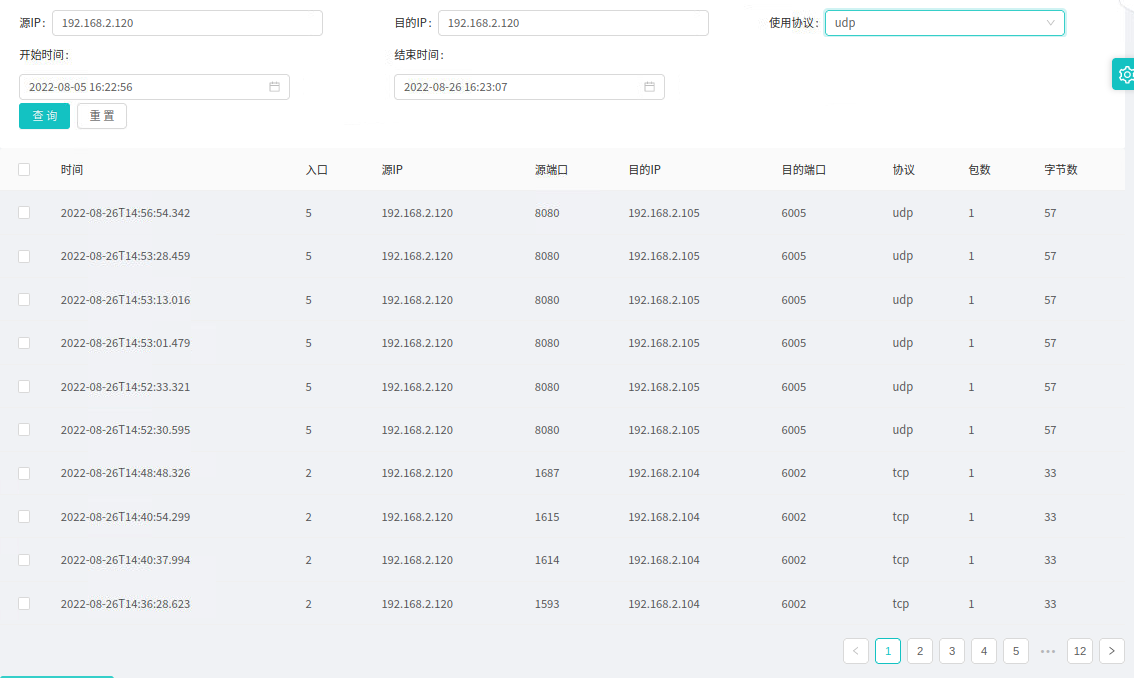
\includegraphics[scale=0.6]{figures/HW/N13.png}
\caption{查询界面}
\end{figure}

编码器的日志查询功能可以通过输入查询参数获得系统中已有的日志列表。其中可供用户选择的参数为,查询日志的关键字、日志的级别、查询的开始时间和查询的结束时间。日志页面如图5.21所示。

\begin{figure}[!htbp]
\centering
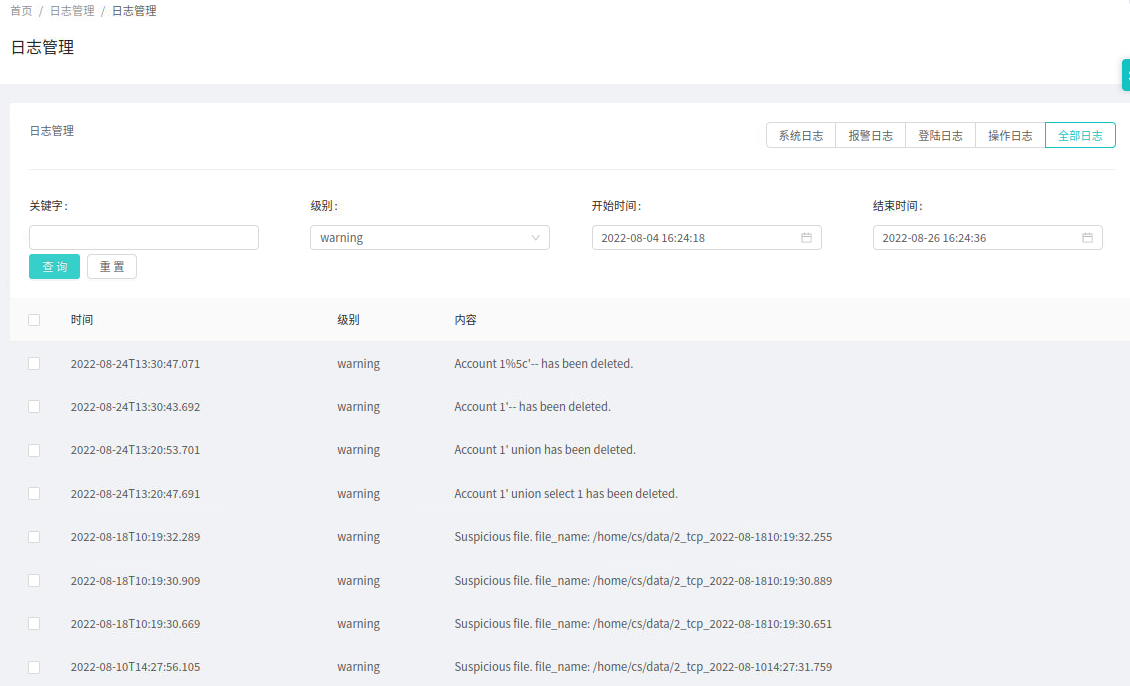
\includegraphics[scale=0.6]{figures/HW/N14.png}
\caption{日志页}
\end{figure}

\section{本章小结}

在本章,我们介绍了与前文提到的基于二维码的传输系统相配套的硬件设备以及控制模块,并且实现了一套可用于用户交互的前后端管理系统。到此为止,我们真正的实现了一台符合工控需求,可以用做单向隔离系统的网闸设备,并且可以在此基础上进行信息的传递。